\section{Optimal Monetary Policy}
\label{sec:MonPol}

Our results so far illustrate that, when BLE and REE are examined under the same set of calibrated parameter values, BLE are characterized by persistence and volatility amplification, with much higher persistence and variance in output gap and inflation compared with REE. As a consequence, there are substantial differences in the estimated parameters and propagation structure when the 3-equation model is evaluated under BLE and REE. This leaves an important question for the optimal Taylor-rule parameters at the BLE. As shown in Boehm and House (2014), at the REE when the output gap and
inflation are observed without error, it is typically optimal to respond infinitely strongly to observed deviation from the central bank's targets, while with measurement error the optimal Taylor rule coefficients are finite.
How do the optimal values of Taylor rule parameters differ between the BLE and REE? In this section we try to answer this question by considering optimal monetary policy under both the calibrated and estimated parameter values. 

Similar to Boehm and House (2014), Evans and Honkapohja (2003) and Woodford (2003), we assume that the central bank wishes to minimize an expected discounted sum of weighted squared inflation and output gap
\begin{equation}
(1-\vartheta)E\Big[\Sigma_{t=0}^\infty \vartheta^t[\omega\pi_t^2+(1-\omega)y_t^2] \Big]=\omega\sigma_\pi^2+(1-\omega)\sigma_y^2,\label{varobj}
\end{equation}
where $\omega$ is the relative weight that the central bank places on inflation. From the equations (\ref{varyapp}) and (\ref{varpiapp}) in Appendix \ref{acfnkc},
\begin{eqnarray}
\sigma_y^2&=&\frac{\widetilde{g}_1}{(1+\gamma\varphi\phi_\pi+\varphi\phi_y)^2(1-\rho^2)(1-\rho\lambda_1)(1-\rho\lambda_2)(1-\lambda_1^2)(1-\lambda_2^2)(1-\lambda_1\lambda_2)}, \label{varyc}\\
\sigma_\pi^2&=&\frac{\widetilde{g}_2}{(1+\gamma\varphi\phi_\pi+\varphi\phi_y)^2(1-\rho^2)(1-\rho\lambda_1)(1-\rho\lambda_2)(1-\lambda_1^2)(1-\lambda_2^2)(1-\lambda_1\lambda_2)}, \label{varpic}
\end{eqnarray}
where $\widetilde{g}_1$, $\widetilde{g}_2$, $\lambda_1$ and $\lambda_2$ are given by the equations (\ref{gyvar}), (\ref{gpivar}), (\ref{lambdatr}) and (\ref{lambdade}). In the following we study the optimal values  $(\phi_y^*, \phi_\pi^*)$ that minimize the central bank's loss function (\ref{varobj}) at the BLE   ($\beta_1^*, \beta_2^*$).

\begin{figure}
    \begin{center}
     \includegraphics[width=3.2in]{optpolicy09.eps}
     \end{center}
   \caption{\label{opt09} Optimal policies at the BLE and at the REE. Parameters are: $\lambda=0.99, \varphi=1, \gamma=0.04, \rho=0.5, \frac{\sigma_2}{\sigma_1}=0.5$ and $\omega=0.9$.}
    \end{figure}
    
    \begin{figure}
    \begin{center}
        \mbox{\subfigure[At the BLE ]
        {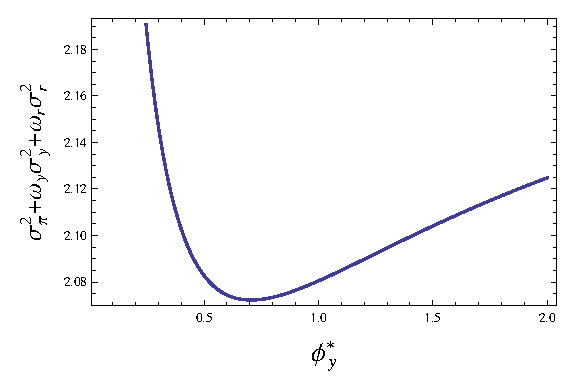
\includegraphics[width=3.2in]{varble09.eps}}\quad
        \subfigure[At the REE]
         {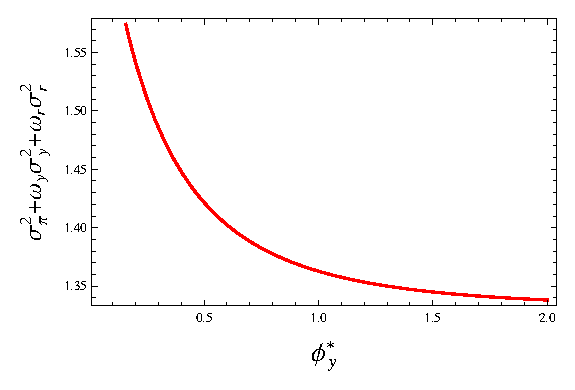
\includegraphics[width=3.2in]{varree09.eps}}}
   \end{center}
   \caption{\label{varopt09} Loss function along the optimal paths $(\phi_y^*, \phi_\pi^*)$ in Figure \ref{opt09} at the BLE (a) and REE (b). Parameters are: $\lambda=0.99, \varphi=1, \gamma=0.04,\rho=0.5, \frac{\sigma_2}{\sigma_1}=0.5$ and $\omega=0.9$.}
    \end{figure}
    
        We first examine monetary policy under BLE and REE at calibrated parameter values: as before in our calibration exercise, we consider the parameters $\lambda=0.99, \varphi=1, \gamma=0.04, \rho=0.5, \frac{\sigma_2}{\sigma_1}=0.5$ for both BLE and REE. This ensures that the economic structure is the same under both specifications, but the implied moments of inflation and output gap are different under BLE and REE.
       We first consider the case $\omega=0.9$, that is, the central bank places relatively large weight on inflation. Interestingly, we find that the optimal Taylor rule coefficients $(\phi_y^*, \phi_\pi^*)$ are finite under BLE in this case\footnote{
We first select a policy parameter domain (e.g. $[0,100]\times[1,100]$) and define a lattice with some small step ($e.g. \,\,0.01$). Then for each lattice point $(\phi_y, \phi_\pi)$, we find the BLE $(\beta_1^*(\phi_y, \phi_\pi), \beta_2^*(\phi_y, \phi_\pi))$ and the corresponding central bank's loss function $\omega\sigma_\pi^2+(1-\omega)\sigma_y^2$ at the BLE. Finally we interpolate the loss function with respect to $(\phi_y, \phi_\pi)$ to find the finite optimal values. It is easy to get analytic expressions of REE and the corresponding variances. In contrast, it is impossible to obtain analytic expressions of the optimal policy parameters under BLE and  therefore we have to rely on numerical approximations. We find consistent results using different ways to calculate the variances (i.e. based on (\ref{varyc}) and (\ref{varpic}) or computing the variances as in Appendix \ref{ACFn}).}.
As shown in Figure \ref{opt09}a, the corresponding optimal policy is $(\phi_y^*, \phi_\pi^*)=(0.9069, 4.8822)$.

This is different from REE, where there is no finite optimal policy except when measurement errors are considered, as shown in Boehm and House (2014). In fact, from Figure \ref{opt09} it can be seen that in the case $\phi_y^*$ is small enough (i.e. $<0.9069$) the coefficients $\phi_y^*$ and $\phi_\pi^*$ lie on a manifold and the loss function (\ref{varobj}) decreases gradually along the manifold within the region, which is similar to REE but with higher $\phi_\pi^*$. However, differently in the case $\phi_y^*>0.9069$, the loss function (\ref{varobj}) starts to increase, while in the REE the loss function (\ref{varobj}) still decreases as shown in Figure~\ref{varopt09}. That is to say, there exist finite optimal Taylor rule coefficients at the BLE, but not at the REE. This is mainly because at the BLE the actual law of motion has higher volatility (especially for inflation) than at the REE in most cases and minimizing the loss function, i.e. minimizing the weighted variances of output gap and inflation, requires balancing the different responses in terms of policy parameters $(\phi_y, \phi_\pi)$.


    
    \begin{figure}
    \begin{center}
        \mbox{\subfigure[Optimal policy ]
        {\includegraphics[width=3.2in]{optpolicyrho09.eps}}\quad
        \subfigure[Optimal manifold]
         {\includegraphics[width=3.2in]{optmanifrho.eps}}}
   \end{center}
   \label{optrho} 
   \caption{ Optimal policies at the BLE with respect to $\rho$ (a) and corresponding optimal manifolds for three different $\rho$ (connection points of solid and dotted curves corresponding to finite optimal policies) (b). Parameters are: $\lambda=0.99, \varphi=1, \gamma=0.04,\frac{\sigma_2}{\sigma_1}=0.5$ and $\omega=0.9$.}
    \end{figure}

Next we investigate how optimal monetary policy changes as the persistence of the underlying shocks is varied. At the REE with measurement error the finite coefficients $\phi_y^*$ and $\phi_\pi^*$ increase as the persistence of shocks grows within some range, see Boehm and House (2014). At the BLE, in addition to this, we find that when the persistence of exogenous shocks becomes sufficiently small with $\rho<0.4$, the finite coefficients $\phi_y^*$ and $\phi_\pi^*$ start increasing as shown in Figure \ref{optrho}a.  Furthermore, Figure \ref{optrho}b suggests that the optimal manifold always moves up as the persistence of shocks $\rho$ grows. The finite optimal policy lies at the point in the optimal manifold connecting the solid and dotted lines in Figure \ref{optrho}b. The location of the optimal point corresponding to finite optimal policies depends on the relative values of variances of output gap and inflation. In the case $\rho$ is large enough, the loss function is mainly dominated by the variance of inflation and hence the optimal policy $\phi_{\pi}^*$ grows quickly converging to $\infty$ and the slope of $\frac{\phi_\pi^*}{\phi_y^*}$ converging to a relatively large constant. Given the parameters, for small enough $\rho$, the loss function is mainly dominated by the variance of the output gap and also the finite optimal policy $\phi_y^*$ grows quickly converging to $\infty$ with a relatively small limit of $\frac{\phi_\pi^*}{\phi_y^*}$. Since both shock persistence parameters are fairly low in our estimation exercise, the optimal pair of coefficients for the U.S. data falls within this region as we will be discussed below. 

In a similar vein, if the weight on inflation $\omega$ is large enough, the loss function is dominated by the variance of inflation. Figure \ref{optomega}a suggests that the optimal policy is $\phi_\pi^*\to\infty$ and $\phi_y^*\to 0$ for $\omega=1$. Therefore, for large enough $\omega$, finite optimal policy $\phi_\pi^*$ increases while  $\phi_y^*$ decreases as $\omega$ grows, as shown in Figure \ref{optomega}. For small enough $\omega$, the variance of output gap plays a dominant role and hence the optimal manifold increases as $\omega$ grows (see Figure \ref{optomega}b). For a range of  $\omega$ values there exist finite optimal policies. As $\omega$ grows, the finite optimal policy $\phi_\pi^*$ first decreases and then increases, while $\phi_y^*$ decreases  within the range of existence of finite optimal policy.




\begin{figure}
    \begin{center}
        \mbox{\subfigure[Optimal policy ]
        {\includegraphics[width=3.2in]{optpolicyomega05.eps}}\quad
        \subfigure[Optimal manifold]
         {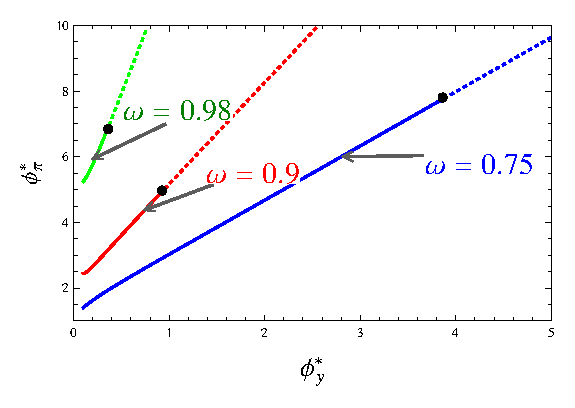
\includegraphics[width=3.2in]{optmanifomega.eps}}}
   \end{center}
   \caption{\label{optomega}  Optimal policies at the BLE with respect to $\omega$ (a) and corresponding optimal manifolds for three different $\omega$ (connection points of solid and dotted curves corresponding to finite optimal policies) (b) with the contemporaneous interest rate rule. Parameters are: $\lambda=0.99, \varphi=1, \gamma=0.04,\frac{\sigma_2}{\sigma_1}=0.5$ and $\rho=0.5$.}
    \end{figure}
    
    \begin{figure}
    \begin{center}
        \mbox{\subfigure[Optimal manifold]
        {\includegraphics[width=3.2in]{optpolicy.eps}}\quad
        \subfigure[Loss function along optimal manifold]
         {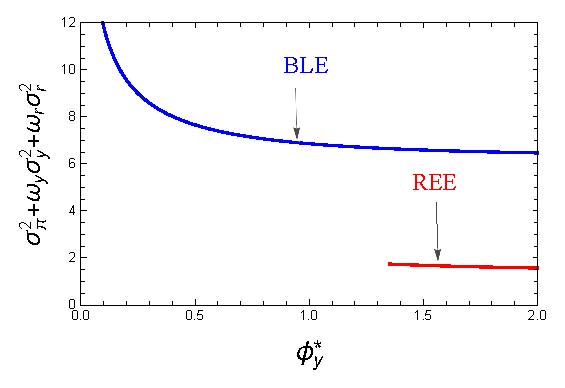
\includegraphics[width=3.2in]{optimalvar.eps}}}
   \end{center}
   \caption{\label{optbench} Optimal manifolds at the BLE and REE given each $\phi_y^*$ (a) and the corresponding loss function along the optimal paths (b) with the contemporaneous interest rate rule. Parameters are: $\lambda=0.99, \varphi=1, \gamma=0.04, \rho=0.5,
\frac{\sigma_2}{\sigma_1}=0.5$ and $\omega=0.5$.}
    \end{figure}

Next we investigate optimal monetary policy at our estimated parameter values. In this case the underlying economic structure is different under BLE and REE, while the moments of inflation and output gap are close under both specifications\footnote{Our analysis with the calibrated values is based on the expressions (3.15)-(3.18). This is no longer applicable since we add interest rate smoothing to our model and relax the assumption that exogenous shocks have the same persistence. Therefore we proceed by computing the fixed-points and the associated variances for each value of policy parameters using our Iterative E-stability algorithm.}. Similar to the calibration exercise, the finite pair of Taylor-coefficients does not exist under REE at the estimated parameter values. While the optimal Taylor-rule is still finite under BLE, the parameter values turn out to be arbitrarily large for both $\phi_y^{*}$ and $\phi_{\pi}^{*}$. This result is already suggested in Figure \ref{optrho}, which shows that optimal coefficients start to rapidly increase when the persistence of exogenous shocks becomes too small. Recalling that our estimated shock persistence parameters are $\rho_y=0.43$ and $\rho_{\pi}=0.32$, the variance of output gap quickly dominates over this region, leading to a large pair of optimal values. The first row of Figure \ref{optim_est} shows how the variances of inflation and output gap change as we vary the monetary policy coefficients over a more empirically plausible range: we vary $\phi_{\pi}$ over $[1,10]$ keeping $\phi_y$ fixed at its estimated value, and $\phi_y$ over $[0,10]$ keeping $\phi_{\pi}$ at its estimated value\footnote{Since the estimated interest rate smoothing parameters are slightly different, we fix this parameter at $\rho_r=0.85$ for both models to make the magnitudes of change in $\phi_{\pi}$ and $\phi_y$ equivalent under BLE and REE.}. It is readily seen that a relatively inactive monetary policy has a destabilizing effect under BLE: when $\phi_{\pi}$ falls below 1, or $\phi_y$ falls below $0.2$, the underlying BLE is destabilized and the variances grow exponentially. This is similar to the standard indeterminacy result under REE, but the negative consequences of a passive monetary policy on the economy are larger under BLE.  These two figures also  show that there is a clear trade-off between inflation and output gap variances when $\phi_{y}$ is kept fixed, while the trade-off with higher values of $\phi_y$ is too small over this empirically plausible range. This also implies that the arbitrarily large pair of optimal coefficients is driven by the small trade-off as $\phi_y$ is varied. 

%This is shown in the left panel of second row in Figure \ref{optim_est}, which plots the optimal values of $\phi_{\pi}$ under BLE and REE as a function of the inflation weight $\omega$.  Since the trade-off between inflation and output gap variance with varying $\phi_{\pi}$ is smaller under BLE, the resulting optimal coefficient also turns out larger  compared with REE for a wide range of weights $\omega$. With a weight of $0.9$,
%the optimal reaction coefficient is $3.57$ under BLE and $1.57$ under REE, with $\phi_{\pi}^{*}\rightarrow\infthy$ as $\omega \rightarrow 1 $ in both cases. 


 \begin{figure}
\centering
       \mbox{\subfigure[Variances w.r.t. $\phi_{\pi}$.]{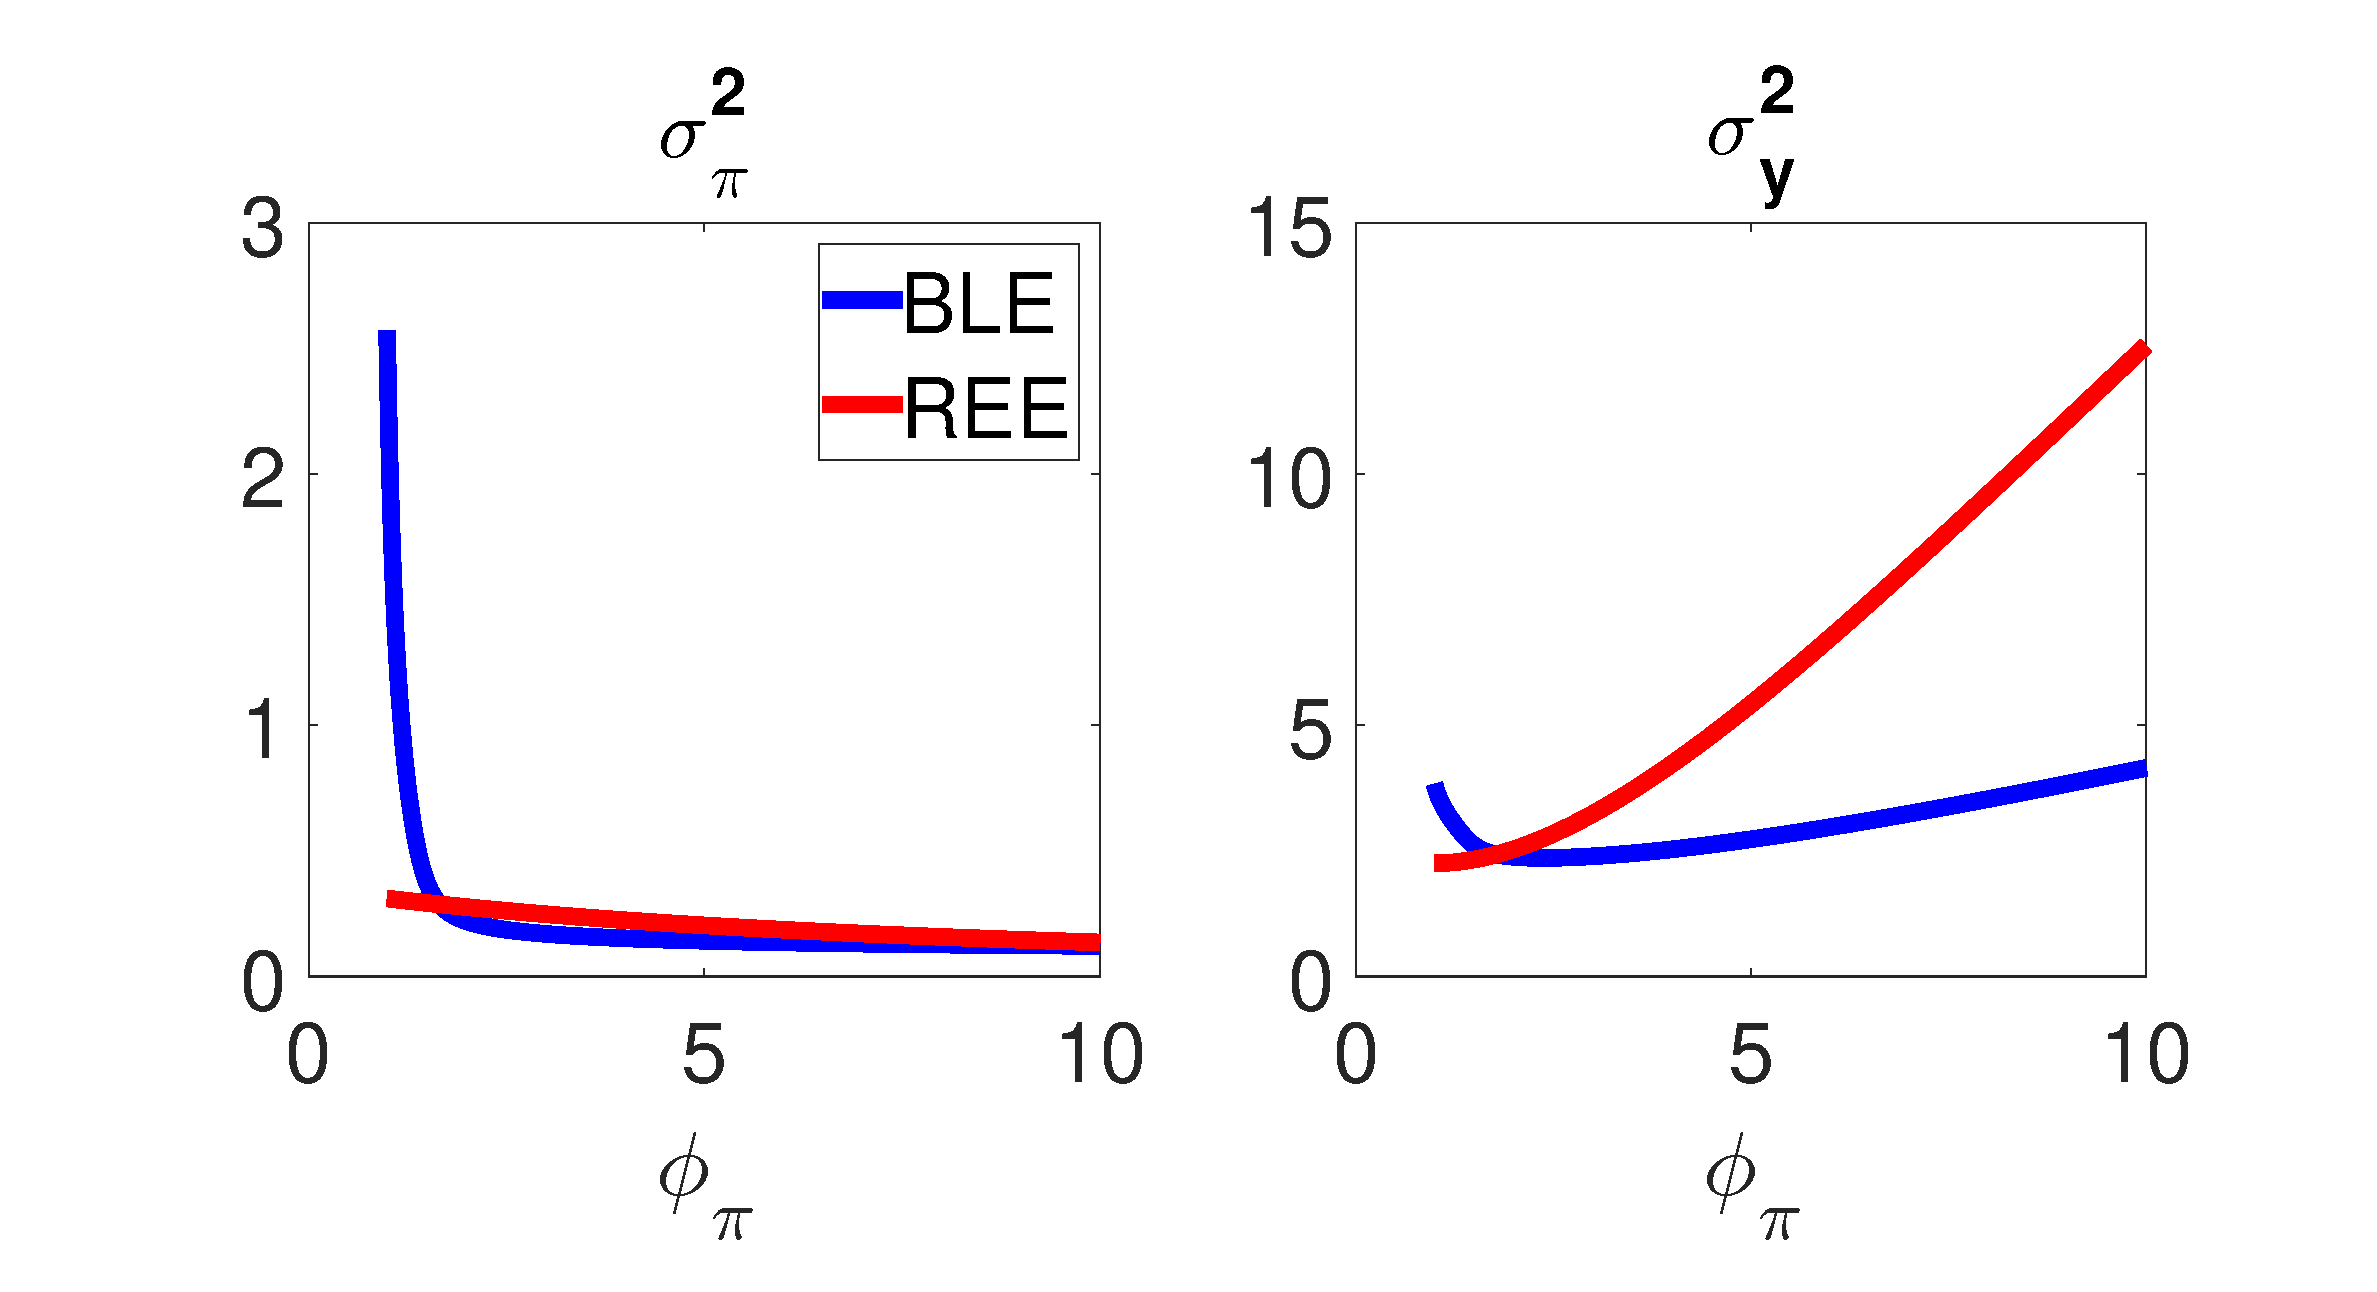
\includegraphics[scale=0.19]{optimal_policy_weight_pi_variances.pdf}}\quad
      \subfigure[Variances w.r.t. $\phi_{y}$.]{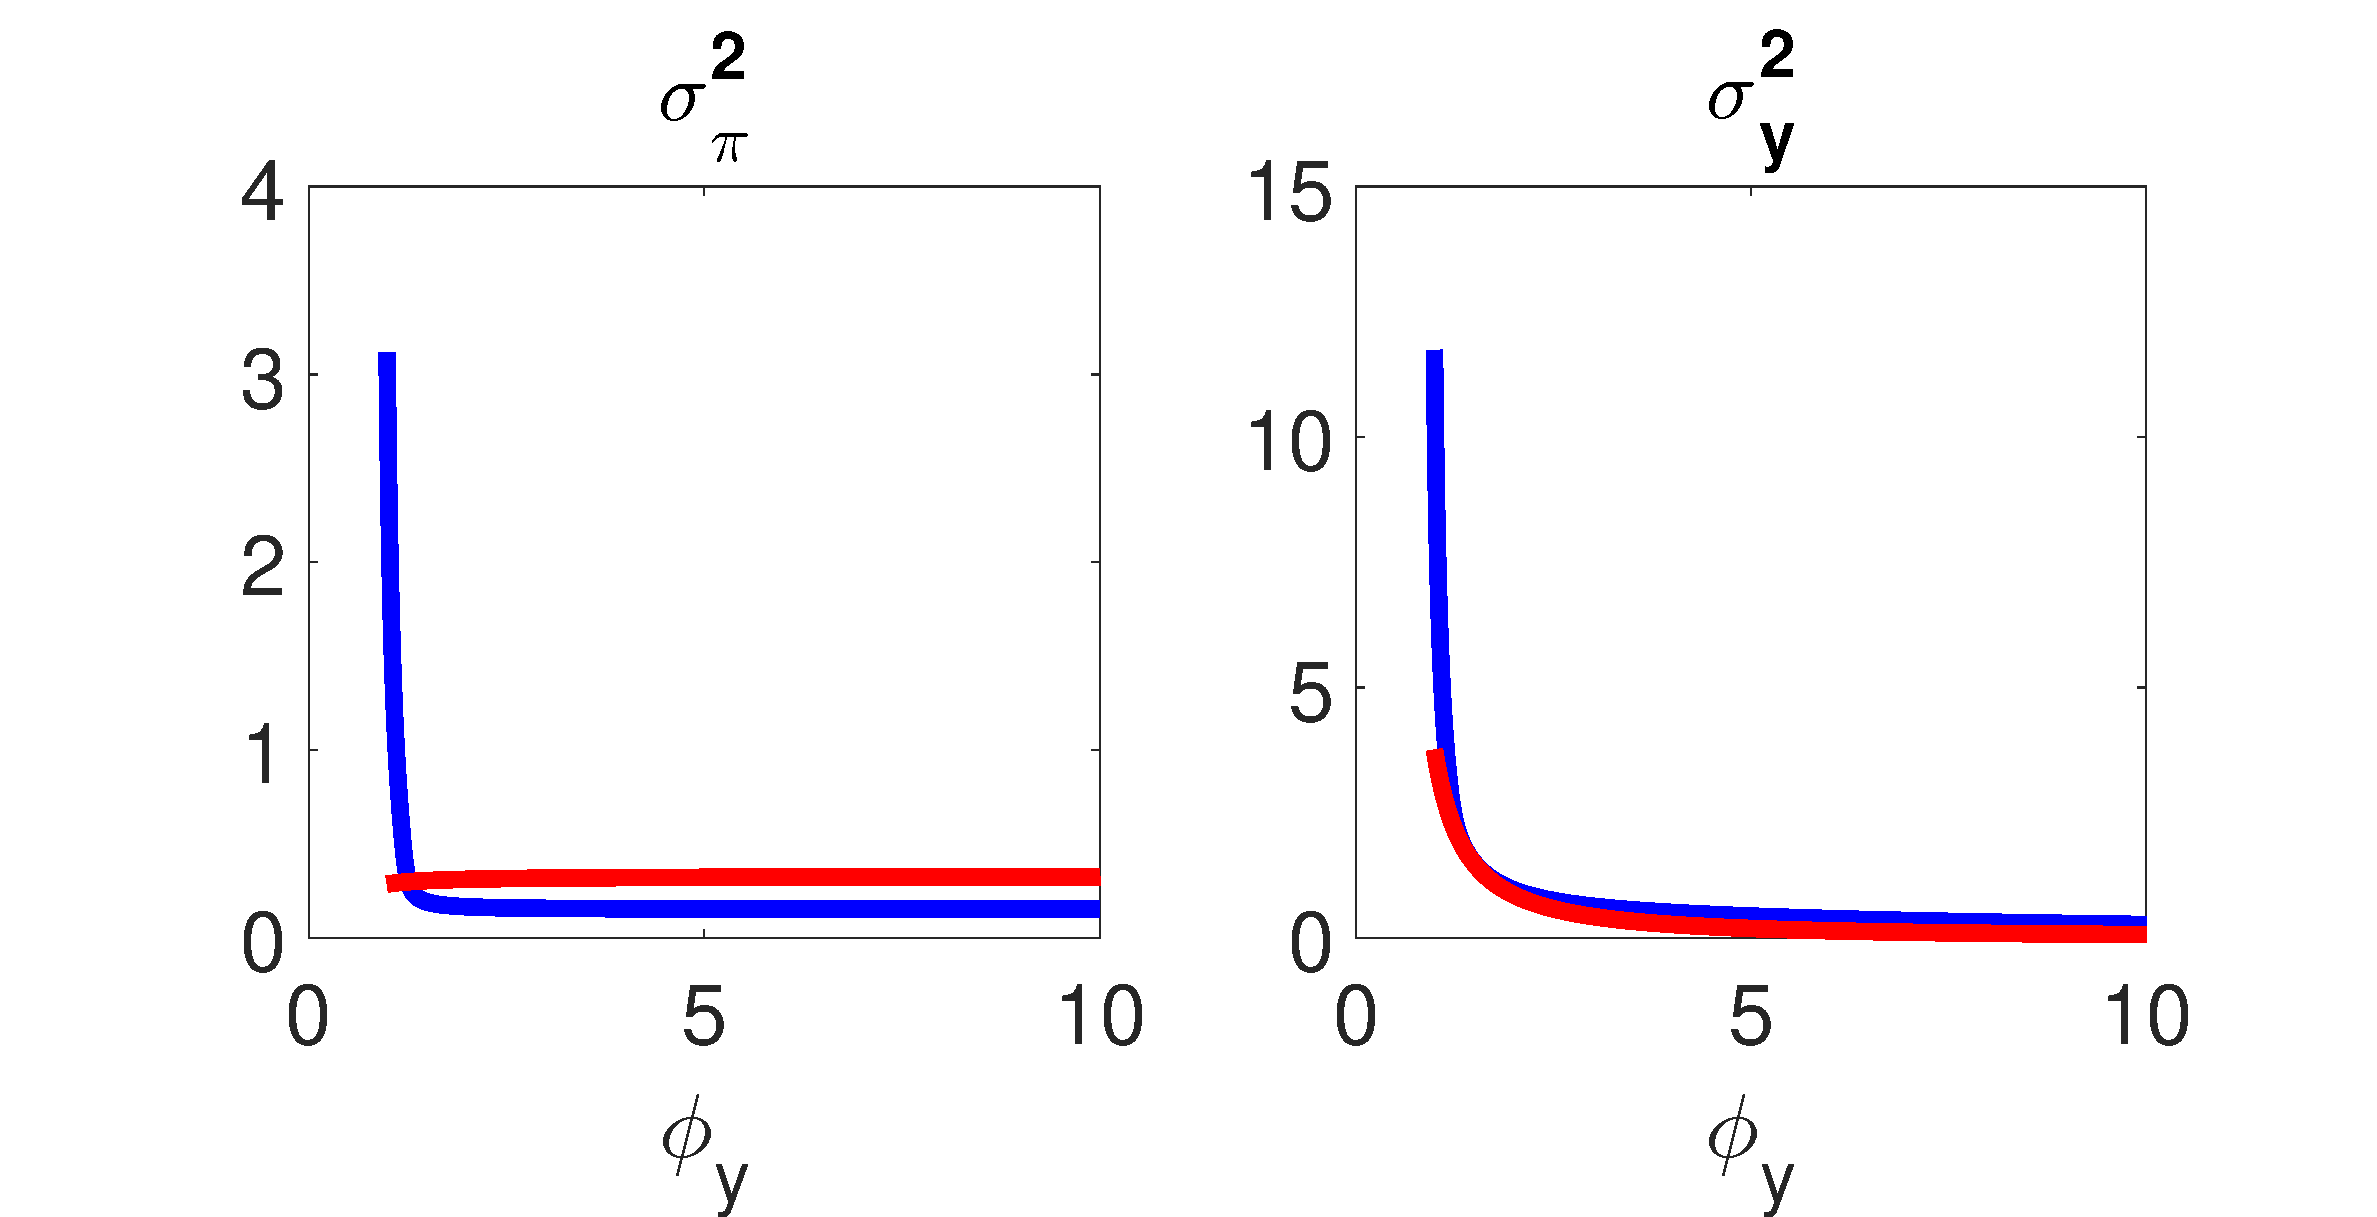
\includegraphics[scale=0.19]{optimal_policy_weight_y_variances.pdf}}}
    \caption{Variances of inflation and output gap as the monetary policy parameters are varied over the empirically plausible range. The blue and red lines show the variances under BLE and REE respectively.}
     \label{optim_est}
 \end{figure}




Figure \ref{imp_resp} shows the impulse responses of inflation and output gap to a monetary policy shock of the same size\footnote{The shock size is one standard deviation at the estimated parameter values for each case, which is the same under BLE and REE with $0.29$.}. Both the initial impact, as well as the cumulative impact of the shock are larger under BLE. This is because both the estimated slope of the Philips curve $\gamma$ and the intertemporal elasticity of substitution $\varphi$ are larger under BLE, leading to a stronger transmission channel of monetary policy shocks compared with REE. Furthermore the shock takes several quarters to reach its full impact under BLE, leading to hump-shaped responses for both inflation and output gap: this shows that the persistence amplification under BLE is also reflected in the system's response to an exogenous monetary policy shock. Together with Figure \ref{optim_est}, this  suggests that monetary policy has a stronger impact on the economy under BLE. 




 
 \begin{figure}
 \centering
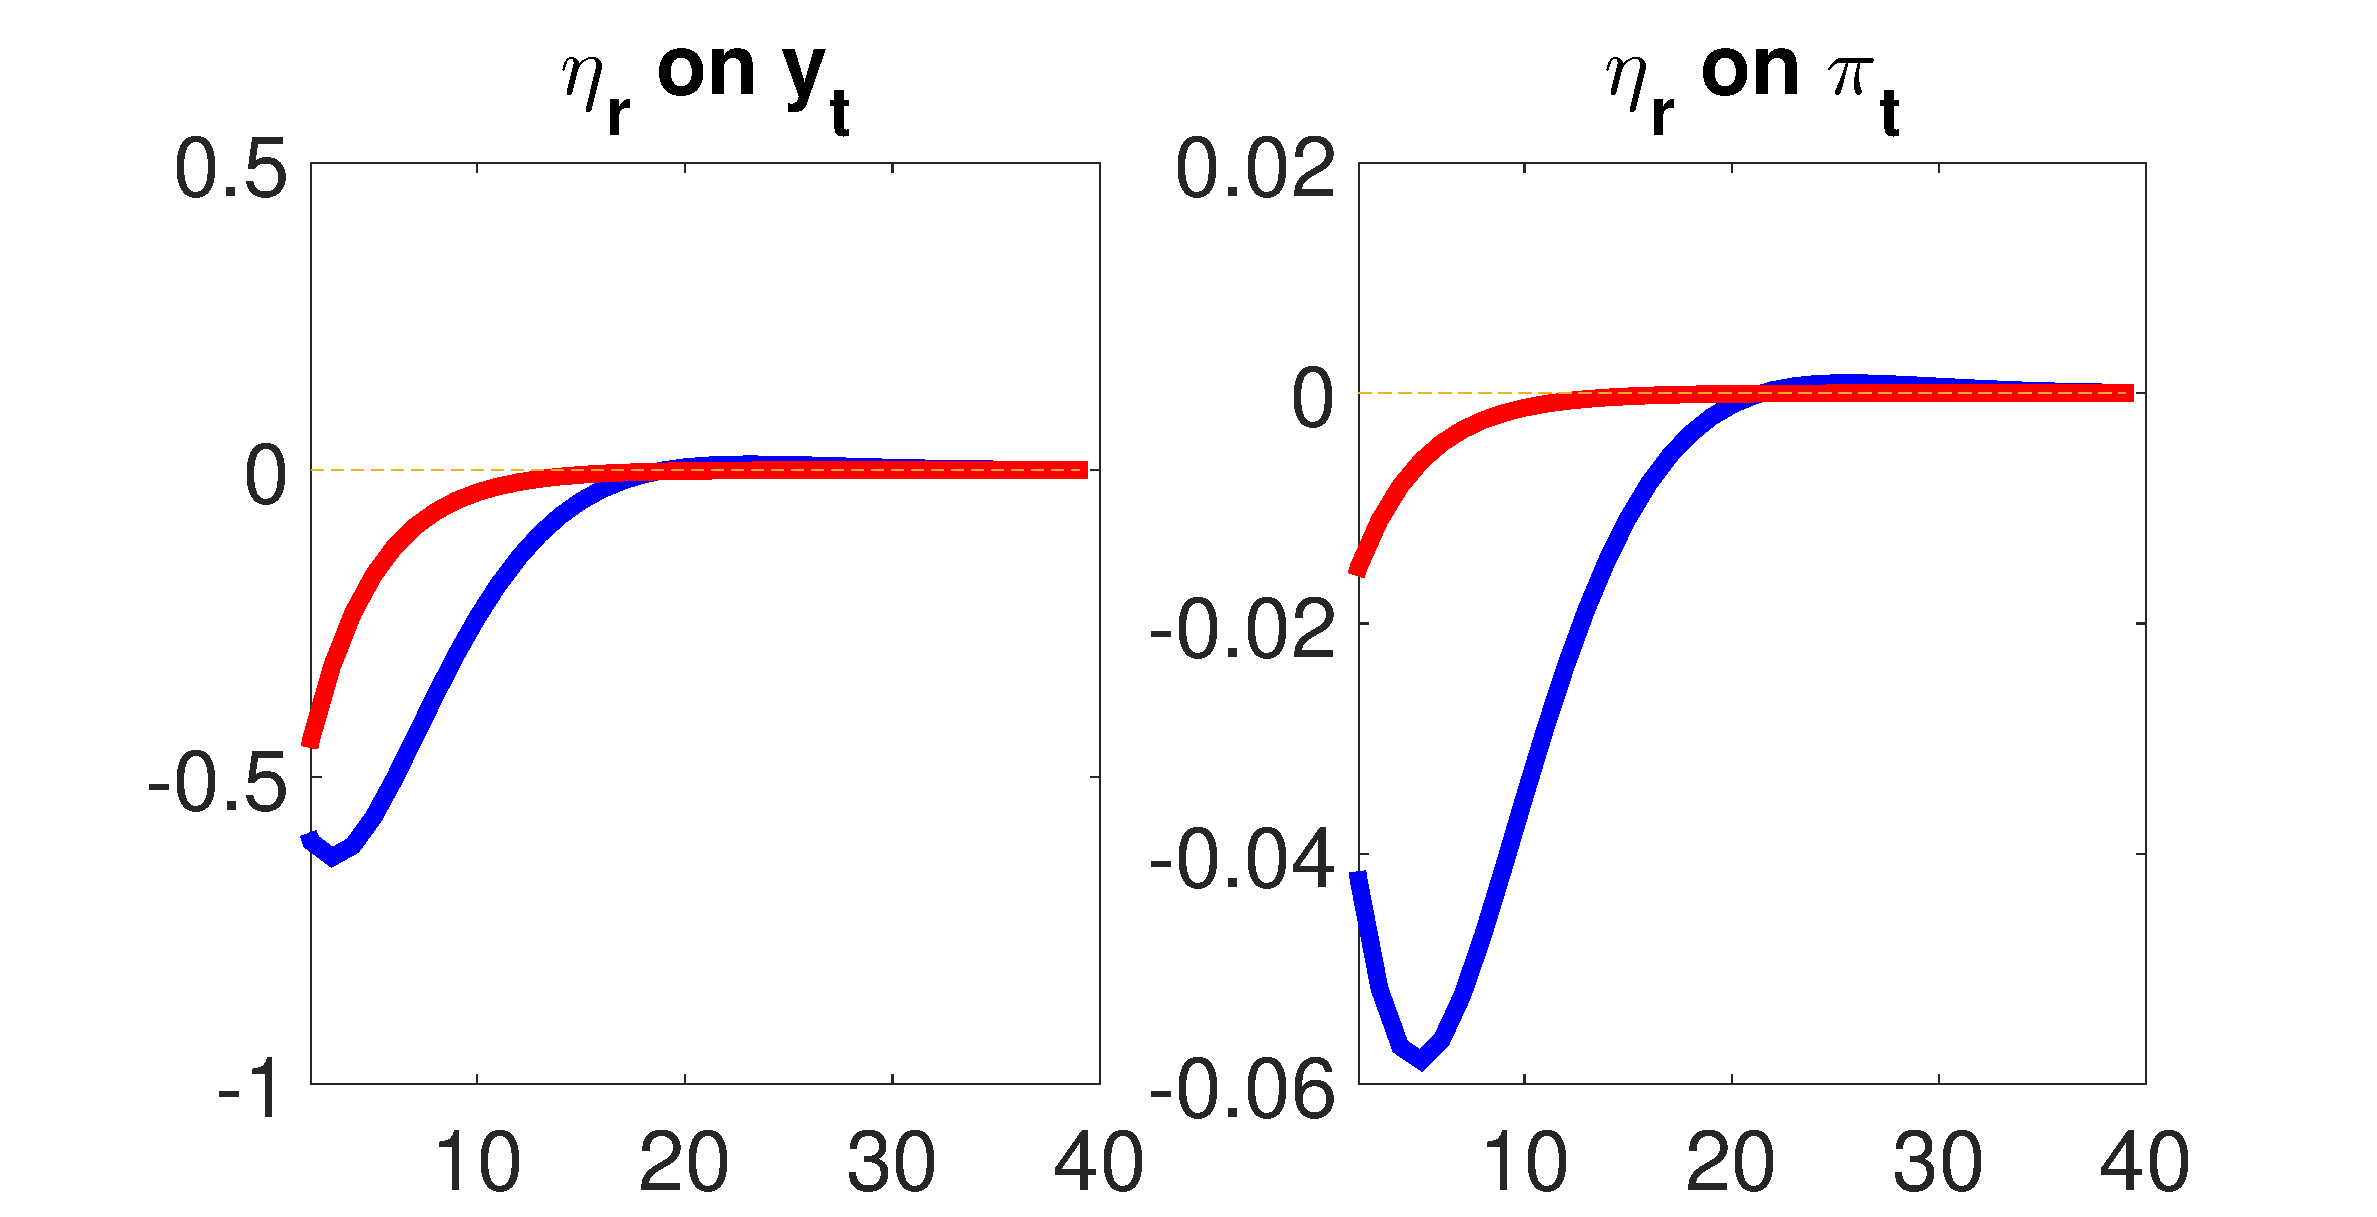
\includegraphics[scale=0.25]{nkpc_irfs_comparison.pdf} 
\caption{Impulse responses to a monetary policy shock of one standard deviation. The blue and red lines show the responses under BLE and REE respectively.}
\label{imp_resp}
\end{figure}
             
 We close this section with an illustration of how multiplicity of equilibria can arise under BLE when monetary policy parameters are varied. In all calibration and estimation exercises that we discussed so far, the underlying BLE is unique. However, multiple stable BLE can arise for certain combinations of parameter values. One such case can be observed when we set the parameter values to their CBO-based output gap estimations as given in Table \ref{nkm_alt_gap}, and vary the values of monetary policy parameters. 

 \begin{figure}
\centering        
             \mbox{\subfigure[Variances $\sigma_y^2$ and $\sigma_{\pi}^2 $ w.r.t. $\phi_{y}$]{\includegraphics[scale=0.19]{phi_y_variance.pdf}   }} 
 \mbox{\subfigure[Variances $\sigma_y^2$ and $\sigma_{\pi}^2 $ w.r.t. $\phi_{y}$]{\includegraphics[scale=0.19]{phi_pi_variance.pdf}}} \\  
            \caption{Optimal Policy under BLE and REE at the estimated parameter values.}
            \label{mult_eqm}
\end{figure}  

In this case the estimated Philips curve slope $\gamma$ is smaller at $0.024$ compared with our benchmark estimation with $\gamma=0.035$. Figure \ref{optim_est} illustrates how inflation and output gap variances change as we vary the monetary policy coefficients $\phi_y \in [0.25, 0.5]$ and $\phi_{\pi} \in [1,1.75]$ in this case. While the change in variances follow the same overall pattern as in the benchmark case, we observe two co-existing E-stable BLE over a small range of parameter values. The underlying BLE is unique at the estimated parameter values, but as the reaction coefficients become smaller, with $\phi_y<0.33$ or $\phi_{\pi}<1.3$, another BLE with higher variance and higher persistence for both inflation and output gap becomes stable and there is a range of parameter values where these two stable BLE co-exist. For smaller values of reaction coefficients,
with $\phi_y < 0.31$ or $\phi_{\pi}<1.1$, 
the low persistence/low variance equilibrium becomes unstable and only the high-variance equilibrium remains. These results suggest that, for certain parameter combinations, there is another important role for monetary policy in terms of ensuring that such high volatility equilibria are destabilized, which is only possible with a sufficiently active policy rule. In our example multiplicity of equilibria is driven by a flatter Philips curve compared to our benchmark case, but similar results can arise when other structural parameters are varied, such as the exogenous shock persistence parameters $\rho_y$ and $\rho_{\pi}$, or the intertemporal elasticity of substitution $\varphi$. \\



